\chapter{State of the art}
\label{chapter:state_of_the_art}

\section{Introduction to reinforcement learning}

Reinforcement learning (RL) is a form of machine learning that can be described as \say{a way of programming agents by reward and punishment without needing to specify how the task is to be achieved} \cite{Kaelbling:1996}. The goal of reinforcement learning is to produce and agent capable of solving a particular problem within an environment. However, the agent has no initial knowledge of the task that it must complete or the effect that its actions have. Instead, it must learn through trial and error by interacting with the environment.

\subsection{Elements}

There are four core elements in a reinforcement learning problem:

\begin{description}
    \item[Agent] The program that makes decisions and takes actions. It must learn what is the best course of action through its experience interacting with the environment.
    \item[Environment] The context that houses the problem to be solved.
    \item[States] Snapshots that describe of the environment at a particular point in time and that the agent uses to make its decisions.
    \item[Reward signal] Real scalar magnitude that the agent needs to maximize in order to achieve its goal.
\end{description}

These elements are described in greater detail below.

\subsubsection{Environment}

\begin{figure}[!h]
    \label{fig:interaction}
    \centering
    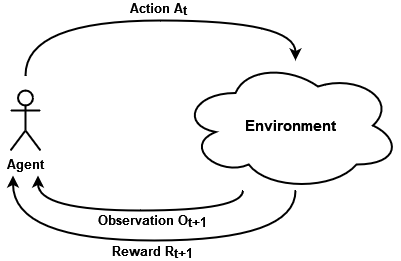
\includegraphics[width=.5\textwidth]{figs/RL_schema.png}
    \caption{Agent-Environment interaction}
\end{figure}

The environment encompasses all that is external to the agent. The agent learns by interacting with the environment in a series of discreet instants, or time steps, as depicted in figure \ref{fig:interaction}. On any given step $t$, the agent:

\begin{enumerate}
    \item receives and observation of the environment $O_t$,
    \item receives a reward $R_t$ based on the current state of the environment, and
    \item executes an action $A_t$.
\end{enumerate}

In response, the environment:

\begin{enumerate}
    \item receives the action $A_t$,
    \item generates a new observation of the environment $O_{t+1}$, and
    \item emits a new reward $R_{t+1}$.
\end{enumerate}

\subsubsection{States}

The states describe the evolution of the environment to reflect the actions taken by the agent. For every time step $t$, the state $S_t$ contains the information of all previous observations, actions and rewards, and can be used to determine how the environment will change in the next time step. Depending on the design of the environment and the agent, the agent may not have perfect knowledge of the sate, meaning that the observation $O_t$ it receives does not equal the true state $S_t$. These environments are called partially observable, as opposed to fully observable environments, in which $O_t = S_t$.

\subsubsection{Reward signal}

The reward signal $R_t$ is a real scalar value that the agent receives after every action it takes. On any given time step $t$, the sum of all future rewards is a random variable $G_t$ known as \textit{return}. The \textit{reward hypothesis} sates that the solution to any problem can be thought as the maximization of the expected value of the return \cite{Sutton:2014}. As such, the agent's goal is to learn actions that maximize the return at the end of the scenario, which doesn't necessarily mean maximizing the immediate reward for the current state. Sometimes it may be necessary to forgo a large immediate reward in favour of greater long-term return.

\begin{equation}
    G_t = R_{t+1} + R_{t+2} + R_{t+3} + \ldots
\end{equation}

Depending on the nature of the environment, it may be the case that the number of steps isn't finite. This could mean that the return never converges. To solve this, a discount value $\gamma \in [0,1]$ is introduced, which reduces the weight of rewards the further away they are from the current time step.

\begin{equation}
    G_t = R_{t+1} + \gamma R_{t+2} + \gamma^2 R_{t+3} + \ldots
\end{equation}

The return can also be expressed recursively:

\begin{align}
\begin{split}
    G_t = &R_{t+1} + \gamma R_{t+2} + \gamma^2 R_{t+3}  + \gamma^3 R_{t+4} + \ldots\\
    &R_{t+1} + \gamma(R_{t+2} + \gamma R_{t+3} + \gamma^2 R_{t+4} + \ldots)\\
    &R_{t+1} + \gamma G_{t+1}
\end{split}
\end{align}

\subsubsection{Agent}

While the previous three elements describe the problem, the agent represents the solution. It is comprised of one or more of the following elements.

\subsubsection*{Policy}

The policy $\pi(\cdot)$ is a function that determines the action that the agent will take in any particular state. There are two types of policies:

\begin{itemize}
    \item \textbf{Deterministic:} The policy maps a single action to each state, meaning that the agent will always take action $a$ when in the state $s$.
    \begin{equation}
        a = \pi(s)
    \end{equation}
    \item \textbf{Stochastic:} The policy assigns one or more actions following a probability distribution to each state. In this case, the policy $\pi(a|s)$ represents the probability that action $a$ will be taken when in the state $s$.
    \begin{equation}
        \pi(a|s) = P(A_t=a|S_t=s)
    \end{equation}
\end{itemize}

\subsubsection*{Value function}

The value function calculates the accumulated future reward (the return) of a state given a policy to follow. This allows us to estimate how \say{good} it is to be in any specific state. There are two approaches:

\begin{itemize}
    \item \textbf{State value function:} It calculates the return of following the policy $\pi$ from the state $s$.
    \begin{align}
    \begin{split}
        v_\pi(s) &= \mathbb{E}_\pi[G_t|S_t = s]\\
        &= \mathbb{E}_\pi[R_{t+1} + \gamma R_{t+2} + \gamma^2R_{t+3} + \ldots|S_t = s]\\
        &= \mathbb{E}_\pi[R_{t+1} + \gamma G_{t+1}|S_t = s]
    \end{split}
    \end{align}
    \item \textbf{Action value function:} It calculates the return of taking the action $a$ (regardless of policy) in the state $s$ and then following the policy $\pi$.
    \begin{align}
    \begin{split}
        q_\pi(s,a) &= \mathbb{E}_\pi[G_t |S_t = s,A_t = a]\\
        &= \mathbb{E}_\pi[R_{t+1} + \gamma R_{t+2} + \gamma^2R_{t+3} + \ldots|S_t = s,A_t = a]\\
        &= \mathbb{E}_\pi[R_{t+1} + \gamma G_{t+1}|S_t = s,A_t = a]
    \end{split}
    \end{align}
\end{itemize}

\subsubsection*{Model}

The model is an internal representation of the environment that the agent uses to try to predict how it will behave. It is an optional element, and agents may or may not have internal models. These models can be of two types:

\begin{itemize}
    \item \textbf{Transition model $\mathcal{P}$:} It estimates, given the current state $s$ and the action to take $a$, the next state $s^\prime$ that the environment will generate.
    \begin{equation}
        \mathcal{P}^a_{ss^\prime} = p(s^\prime|s,a) \approx P(S_{t+1} = s^\prime|S_t = s, A_t = a)
    \end{equation}
    \item \textbf{Reward model $\mathcal{R}$:} It approximates the reward that the agent will receive when performing the action $a$ in the state $s$.
    \begin{equation}
        \mathcal{R}^a_s = r(s,a) \approx \mathbb{E}[R_{t+1}| S_t = s, A_t = a]
    \end{equation}
\end{itemize}

\subsection{Challenges in reinforcement learning}
\label{sec:challenges}

Next, we introduce some of the common challenges that are found in RL.

\subsubsection*{Learning and planning}

There are two main configuration of sequential decision-making problems. The first is reinforcement learning in the strict sense, where the environment is unknown to the agent, which must interact with it and improve its policy by trial and error. In the second, planning, the agent starts with a perfect model of the environment and uses it to calculate improvements to the policy.

These approaches a usually separated, but they may sometimes be related, for example in problems where reinforcement learning is used to create a model of the environment which is then used in planning.

\subsubsection*{Exploration and exploitation}

Exploration is the process by which the agent finds new paths or alternative courses of action that allow it to discover better solutions. Exploitation is the process of using the best known solutions to maximize the reward. As such, there is a balance to be found between the two, since both are necessary to solve the problem: the agent should work on optimizing the most promising solutions, but also keep exploring alternatives.

\subsubsection*{Prediction and control}

A prediction is the concept of evaluating the future based on a policy $\pi$, such as predicting the return with a value function $v_\pi(s)$. Control refers to optimizing the future, for example, by finding the optimal policy $\pi_\ast(s)$ that would generate the greatest return. These concepts are related as follows:

\begin{equation}
    \pi_\ast(s) = \underset{\pi}{\operatorname{argmax}}\,v_\pi(s)
\end{equation}

The optimal policy is the one that results in the maximum value function. Typically, in reinforcement learning problems, is necessary to first solve the prediction problem by estimating $v_\pi(s)$ in order to solve the control problem, since the value function is used to evaluate and compare different policies.

\section{Definition of the problem}

A reinforcement learning problem can be described as a Markov decision process \cite{Sutton:2014}, which is defined by the tuple $<\mathcal{S}, \mathcal{A},\mathcal{P},\mathcal{R},\gamma>$.

\begin{description}
    \item[$\mathcal{S}$] is the finite set of all possible states in the environment ($S_t \in \mathcal{S}$). These states follow the \textit{Markov property} (equation \ref{eq:markov}), which means that the evolution of a state depends only on that state, and is independent of all the previous ones \cite{Sutton:2014}.
    \begin{equation}
    \label{eq:markov}
        P(S_{t+1}|S_t) = P(S_{t+1}|S_1, S_2, \ldots, S_t)
    \end{equation}
    \item[$\mathcal{A}$] is the finite set of all possible actions that the agent can take ($A_t \in \mathcal{A}$).
    \item[$\mathcal{R}$] is the finite set of all possible rewards ($R_t \in \mathcal{R}$). 
    \item[$\mathcal{P}$] is the state transition matrix, which contains the probabilities for all the transition from a state $s$ to the next state $s^\prime$. Its elements can be of one of two forms, depending on whether the reward for the transition is deterministic (equation \ref{eq:transition_det}) or stochastic (equation \ref{eq:transition_sto}).
    \begin{equation}
    \label{eq:transition_det}
        p(s^\prime|s, a) = P(S_{t+1} = s^\prime|S_t = s, A_t = a)
    \end{equation}
    \begin{equation}
    \label{eq:transition_sto}
        p(s^\prime, r|s, a) = P(S_{t+1} = s^\prime, R_{t+1} = r|S_t = s, A_t = a)
    \end{equation}
    \item[$\gamma$] is the discount value applied to the rewards when calculating the return.
\end{description}

Once these elements are defined, the expected value of the rewards used by the value functions can be calculated.

\begin{align}
\begin{split}
    \label{eq:bellman_state}
    v_\pi(s) &= \mathbb{E}_\pi[R_{t+1} + \gamma G_{t+1}|S_t = s] \\
    &= \sum_{\forall a \in \mathcal{A}}{\pi(a|s)} \sum_{\substack{\forall r \in \mathcal{R} \\ \forall s^\prime \in \mathcal{S}}}{p(r,s^\prime|s,a)[r + \gamma v_\pi(s^\prime)]}
\end{split}
\end{align}

\begin{align}
\begin{split}
    \label{eq:bellman_action}
    q_\pi(s,a) &= \mathbb{E}_\pi[R_{t+1} + \gamma G_{t+1}|S_t = s, A_t = a] \\
    &= \sum_{\substack{\forall r \in \mathcal{R} \\ \forall s^\prime \in \mathcal{S}}}{p(r,s^\prime|s,a)[r + \gamma \sum_{\forall a \in \mathcal{A}}{\pi(a^\prime|s^\prime)q_\pi(s^\prime,a^\prime)}]}
\end{split}
\end{align}

\section{Solutions}

To solve a reinforcement learning problem it is necessary to find the optimal state value function $v_\ast(s)$ and optimal action value function $q_\ast(s,a)$. These are the value functions that return the greatest value from all policies.

\begin{equation}
    v_\ast(s) = \max_{\pi}{v_\pi(s)}
\end{equation}

\begin{equation}
    q_\ast(s,a) = \max_{\pi}{q_\pi(s,a)}
\end{equation}

These functions are related in that the optimal state value function of a state $s$ will be equal to the optimal action value function when selecting the action $a$ that maximizes the return in that state.

\begin{equation}
    v_\ast(s) = \max_{a}{q_\ast(s,a)}
\end{equation}

Knowing these functions is enough to solve the environment, since they instantly lead to the optimal policy $\pi_\ast$, which is the policy that maximizes the return of every possible state. This policy can be obtained from the optimal action value function by following the action with the greatest return.

\begin{equation}
    \pi_\ast(a|s) = 
    \begin{cases}
        1 &\textrm{if $a = \underset{a \in \mathcal{A}}{\operatorname{argmax}}$}\,q_\ast(s,a)\\
        0 &\textrm{otherwise}
    \end{cases}
\end{equation}

The solution for the optimal value functions can be obtained by maximizing the actions in the equations \ref{eq:bellman_state} and \ref{eq:bellman_action}.

\begin{equation}
    v_\ast(s) = \max_{a} \sum_{\substack{\forall r \in \mathcal{R} \\ \forall s^\prime \in \mathcal{S}}}{p(r,s^\prime|s,a)[r + \gamma v_\ast(s^\prime)]}
\end{equation}

\begin{equation}
    q_\ast(s,a) = \sum_{\substack{\forall r \in \mathcal{R} \\ \forall s^\prime \in \mathcal{S}}}{p(r,s^\prime|s,a)[r + \gamma \max_{a^\prime} q_\ast(s^\prime,a^\prime)]}
\end{equation}

\subsection{Q-Learning}

Q-Learning \cite{Watkins:1992} is a common control algorithm for approximating the optimal action value function. This algorithm estimates $q_\ast$ via a function $Q(s,a)$. The agent interacts with the environment following a greedy policy based on the current value of $Q$: $\pi_\textrm{greedy}(s) = \max_a Q(s,a)$. On every step $t$, the value of $Q$ is updated with the following formula, where the step size constant (or learning rate) $\alpha \in [0,1)$ determines the magnitude of each update:

\begin{equation}
    Q(S_t,A_t) = Q(S_t,A_t) + \alpha[R_{t+1} + \gamma \max_a Q(S_{t+1},a) - Q(S_t,A_t)]
\end{equation}

In this formula, the term $R_{t+1} + \gamma \max_a Q(S_{t+1},a) - Q(S_t,A_t)$ is called the \textit{temporal difference error} (TD error, $\delta_t$) and represents the difference between the current estimation of $Q(S_t,A_t)$ and the new estimation after step $t$ (also known as target).

\subsection{Deep Q-Learning}

A problem of the Q-Learning algorithm is that the estimator function $Q$ acts as a table that holds the approximated value of $q_\ast$ for every combination of state and action, meaning that, for an environment with $m$ possible states and $n$ actions, the size of the table would be $m \times n$. 

The \textit{curse of dimensionality} is a known problem caused by the fact that the number of states in an environment grows exponentially with the number of variables \cite{Bellman:1957}. For environments with a large number of possible states, such as those where the state is determined by one or more discreet values, it quickly becomes unfeasible to store a value for each combination, both in terms of memory space and computing power.

One way to tackle this issue is to use an artificial neural network as a non-linear estimator for the value function. This combination of deep learning and reinforcement learning is called \textit{deep reinforcement learning} (DRL). When this strategy is applied to the Q-Learning algorithm it is known as \textit{deep Q-Learning} (DQN) \cite{Mnih:2013}. In this new algorithm (shown in algorithm \ref{alg:dqn1}), a neural network $Q_\theta$ with randomly initialized weights $\theta$ is used to approximate the value function. The agent takes actions following a greedy policy $\pi_\textrm{greedy}(s) = \max_a Q_\theta(s,a)$ and after every step a target value is calculated. This target value represents the new estimation of the value function for the action taken $Q_\theta(S_t, A_t)$. This value and the difference to the current inference estimation are used to calculate the loss that will be used to update the network via gradient descent and backpropagation.

\subsubsection*{$\epsilon$-greedy method}

Although powerful, deep Q-Learning is still subject to the common challenges of reinforcement learning, such as the problem of exploration vs exploitation described in section \ref{sec:challenges}. The $\epsilon$-greedy method consists in using a probability parameter $\epsilon \in [0,1]$ to control how frequently the agent explores the environment by taking random actions versus exploiting it by following the learned policy. $\epsilon$ begins with value equal or close to $1$ and decreases as the training progresses. This allows the agent to take mostly random actions at the beginning, when it has little to no knowledge of the environment, and take actions based on what it has learned later on.

The equation \ref{eq:eps} describes an $\epsilon$-greedy policy.

\begin{equation}
\label{eq:eps}
    \pi(a|s) =
    \begin{cases}
        1-\epsilon + \frac{\epsilon}{|\mathcal{A}(s)|} & \textrm{if $a = \underset{a}{\operatorname{argmax}}\,Q(s, a)$}\\
        \frac{\epsilon}{|\mathcal{A}(s)|} & \textrm{if $a \neq \underset{a}{\operatorname{argmax}}\,Q(s, a)$}
    \end{cases}
\end{equation}

\subsubsection*{Experience replay buffer}

A requirement to apply stochastic gradient descent to a neural network is that the data-points must be independently and identically distributed (i.i.d.). But that is not the case for the data of the steps that are traversed by the agent during training. Whenever the agent interacts with the environment, the future state will be a direct consequence of the current state and the selected action, meaning that the explored states are strongly correlated.

A technique to solve this issue is known as the experience replay buffer. It consists in using a large buffer with fixed size to store previous experiences. Before the training begins, the agent is made to randomly explore the environment, storing the experiences (consisting of the current state, the selected action, the reward obtained and the next state: $(S_t, A_t, R_t, S_{t+1})$) in the buffer until it is full. Then, during training, instead of using the most recent experience to update the network, a random subset of the buffer is used. And as the agent explores new states, these are saved to the buffer, replacing the oldest experiences. This process allows the agent to learn from experiences considerably more independent of each other, while still being introduced to later experiences as the process advances and the older ones in the buffer are replaced.

\subsubsection*{Target network}

Another problem in DQL is that the target value of the network is constantly changing, since it depends on the network itself, witch gets updated every step. This causes a great deal of instability during training, and makes it harder for the network to converge. To avoid this problem, a second neural network $\hat{Q}_{\theta^-}$ with the same structure as the prediction network $Q_\theta$ is introduced. This network, called the \textit{target network}, becomes the one used to calculate the target value that is then used to obtain the loss. The target network is originally identical to the main network (has the same weights), but it is not updated on every step like the main one. Instead, after a certain number $N$ of steps, the target network is synchronized with the prediction network by simply cloning its weights. This means that for $N$ iterations, the target $\hat{Q}_{\theta^-}(s^\prime, a^\prime)$ will not be affected by the change to the prediction network $Q_\theta$, which results in more stability during training.

\subsubsection*{Final DQN algorithm}

Algorithm \ref{alg:dqn2} shows what Deep Q-Learning looks like after the aforementioned techniques are implemented \cite{Mnih:2015}.

\subsection{Hierarchical reinforcement learning}

Hierarchical reinforcement learning (HRL) is the strategy of dividing the main problem into several sub-problems, which are then learned by a hierarchy of agents trained by reinforcement learning \cite{Barto:2003, Al-Emran:2015, Pateria:2021}. This hierarchy typically sees a number of low-level agents learn only one specific subtask, but these agents don't choose when they get to act. Instead, a higher-level agent decides what subtask to pursue at any given point, essentially using its actions to select which lower-level agent gets to interact with the environment. Depending on the complexity of the problem, this hierarchy may have an arbitrary number of abstraction layers.

By tackling several subtasks with reduced complexity, HRL helps mitigate the curse of dimensionality. Additionally the use of independent agents brings the additional benefit of greater modularity and reusability of the solutions \cite{Al-Emran:2015}.